\chapter{Balanced Networks}
\label{ch:balanced-networks}

\textit{Balanced networks explain how cortical-like circuits can fire irregularly without slow latent state switching. Excitation and inhibition are individually large, but feedback keeps their residual near threshold. This produces fast asynchronous irregular spiking, not by itself clustered metastability.}

\begin{aside}[Citation TODO]
Add exact citations for classical balanced-network theory only after the bibliography is verified by the final coordinator. This chapter uses standard mechanism-level facts: strong excitation and inhibition cancel in the mean, residual fluctuations drive irregular spiking, and unstructured balanced networks are the control case for clustered metastability.
\end{aside}

% ============================================================
\section{Excitation-inhibition balance}
\label{sec:excitation-inhibition-balance}
% ============================================================

Excitation-inhibition balance is an operating regime of a recurrent network. It is not the statement that every excitatory synapse is paired with an inhibitory synapse. It is the statement that the total excitatory input and total inhibitory input to a neuron are both large, while their sum is much smaller than either component.

For a neuron $i$, decompose the recurrent input into excitatory and inhibitory parts:
%
\begin{equation}
  I_i^{\mathrm{rec}}(t)
  =
  I_i^E(t)+I_i^I(t),
  \qquad
  I_i^E(t)>0,
  \qquad
  I_i^I(t)<0 .
  \label{eq:ei-input-decomposition}
\end{equation}
%
The balanced regime is
%
\begin{keyequation}[Balance as Cancellation]
\begin{equation}
  I_i^E(t)+I_i^I(t)+I_i^{\mathrm{ext}}(t)
  =
  \text{small residual drive},
  \qquad
  |I_i^E|,\ |I_i^I|
  \gg
  |I_i^E+I_i^I+I_i^{\mathrm{ext}}|.
  \label{eq:balance-cancellation-ch04}
\end{equation}
\tcblower
Large excitation pushes voltage upward; large inhibition pulls it downward; the residual determines whether the neuron sits near threshold.
\end{keyequation}

\noindent At the population level, let $a,b\in\{E,I\}$ denote the postsynaptic and presynaptic cell classes. If a neuron in population $a$ receives $K_{ab}$ inputs from population $b$, with synaptic weight $J_{ab}$ and presynaptic rate $r_b$, then a mean-input approximation is
%
\begin{equation}
  \mu_a
  =
  I_a^{\mathrm{ext}}
  +
  \sum_{b\in\{E,I\}}K_{ab}J_{ab}r_b .
  \label{eq:balanced-mean-input-ch04}
\end{equation}
%
Here $J_{aE}>0$ and $J_{aI}<0$ under a signed-current convention. The mean input $\mu_a$ changes when external drive changes, when recurrent rates change, or when the connectivity statistics change.

The balance equations are the approximate conditions that keep $\mu_a$ in a firing-compatible range rather than letting it grow with the number of inputs:
%
\begin{equation}
  I_a^{\mathrm{ext}}
  +
  \sum_{b\in\{E,I\}}K_{ab}J_{ab}r_b
  =
  O(1),
  \qquad
  a\in\{E,I\}.
  \label{eq:balance-equations-ch04}
\end{equation}
%
These equations do not fix spike timing. They fix the mean operating point. The irregular spike timing comes from fluctuations around that point.

The practical implication is that an unclustered balanced network is the correct control model for this course. Before invoking clusters, one should verify that the same neuron and synapse model can produce plausible mean rates and irregular spiking in a random E/I network.

% ============================================================
\section{Current-based vs conductance-based models}
\label{sec:current-vs-conductance-balanced}
% ============================================================

Balanced-network theory is often introduced with current-based synapses because the algebra is transparent. In a current-based LIF network,
%
\begin{equation}
  \tau_m\dot V_i
  =
  -(V_i-E_L)
  +
  R_m\left[
    I_i^{\mathrm{ext}}(t)
    +
    \sum_j J_{ij}x_j(t)
  \right].
  \label{eq:current-based-balanced-lif}
\end{equation}
%
The filtered presynaptic variable $x_j$ is multiplied by a fixed signed weight $J_{ij}$. The effect of a presynaptic spike does not depend on postsynaptic voltage.

In a conductance-based model,
%
\begin{equation}
  C_m\dot V_i
  =
  -g_L(V_i-E_L)
  -
  g_i^E(t)(V_i-E_E)
  -
  g_i^I(t)(V_i-E_I)
  +
  I_i^{\mathrm{ext}}(t).
  \label{eq:conductance-based-balanced-lif}
\end{equation}
%
The conductances $g_i^E$ and $g_i^I$ are nonnegative filtered sums of excitatory and inhibitory presynaptic spikes. The reversal potentials $E_E$ and $E_I$ determine the direction of current. Excitatory conductance usually drives $V_i$ toward a depolarized reversal level, while inhibitory conductance drives or clamps it near a hyperpolarized or shunting level.

Equation \cref{eq:conductance-based-balanced-lif} can be rewritten to expose the effective time constant:
%
\begin{equation}
  C_m\dot V_i
  =
  -g_i^{\mathrm{tot}}(t)
  \left[
    V_i-E_i^{\mathrm{eff}}(t)
  \right]
  +
  I_i^{\mathrm{ext}}(t),
  \label{eq:conductance-effective-form}
\end{equation}
%
where
%
\begin{equation}
  g_i^{\mathrm{tot}}
  =
  g_L+g_i^E+g_i^I,
  \qquad
  E_i^{\mathrm{eff}}
  =
  \frac{g_L E_L+g_i^E E_E+g_i^I E_I}{g_i^{\mathrm{tot}}}.
  \label{eq:conductance-effective-quantities}
\end{equation}
%
Increasing conductance decreases the effective membrane time constant,
%
\begin{equation}
  \tau_i^{\mathrm{eff}}(t)
  =
  \frac{C_m}{g_i^{\mathrm{tot}}(t)}.
  \label{eq:conductance-effective-time-constant}
\end{equation}
%
Thus conductance-based balance has two effects: cancellation of depolarizing and hyperpolarizing drives, and shunting through increased total conductance.

For the rotation, current-based models are useful for first reproductions and analytic reductions. Conductance-based models are important when the question involves voltage variance, shunting inhibition, or the distinction between current variability and membrane-potential variability.

% ============================================================
\section{Strong coupling and cancellation of large inputs}
\label{sec:strong-coupling-cancellation}
% ============================================================

The word balanced becomes mathematically sharp in the strong-coupling limit. Suppose each neuron receives $K$ recurrent inputs. The generic weight $J_{ab}$ in \cref{eq:balanced-mean-input-ch04} is now split into an actual individual synaptic weight and an order-one coefficient:
%
\begin{equation}
  w_{aE}
  =
  \frac{j_{aE}}{\sqrt K},
  \qquad
  w_{aI}
  =
  -\frac{j_{aI}}{\sqrt K},
  \qquad
  j_{ab}=O(1),
  \qquad
  j_{aI}>0 .
  \label{eq:strong-coupling-weight-scaling}
\end{equation}
%
Here $w_{ab}$ is the actual signed synaptic weight from population $b$ to population $a$. The coefficient $j_{ab}$ is positive for both excitation and inhibitory strength; the minus sign in $w_{aI}$ carries the inhibitory sign. If $K_{ab}=\alpha_{ab}K+O(1)$ with $\alpha_{ab}=O(1)$, the total excitatory and inhibitory currents can each be of order $\sqrt K$, while their difference remains order one.

A schematic input to population $a$ is
%
\begin{equation}
  \mu_a
  =
  \sqrt K
  \left(
    \alpha_{aE}j_{aE}r_E
    -
    \alpha_{aI}j_{aI}r_I
    +
    i_a^{\mathrm{ext}}
  \right)
  +
  O(1),
  \label{eq:strong-coupling-mean-input}
\end{equation}
%
where the actual external drive has been written as $\sqrt K\,i_a^{\mathrm{ext}}+O(1)$. Thus $i_a^{\mathrm{ext}}$ is the external-drive coefficient after the leading $\sqrt K$ scale has been extracted, not the unscaled external current in \cref{eq:balanced-mean-input-ch04}. To keep $\mu_a=O(1)$ as $K$ grows, the leading term must nearly vanish:
%
\begin{equation}
  \alpha_{aE}j_{aE}r_E
  -
  \alpha_{aI}j_{aI}r_I
  +
  i_a^{\mathrm{ext}}
  \approx
  0,
  \qquad
  a\in\{E,I\}.
  \label{eq:leading-balance-condition}
\end{equation}
%
This pair of equations determines the mean rates required for cancellation, if the resulting rates are positive and dynamically stable.

The same scaling leaves fluctuations large enough to matter. Under an independent-input approximation, the input variance has the form
%
\begin{equation}
  \begin{aligned}
  \sigma_a^2
  &=
  \sum_{b\in\{E,I\}}
  K_{ab}w_{ab}^2 r_b
  \int_0^\infty\kappa_{ab}^2(t)\,\dd t
  \\
  &=
  \sum_{b\in\{E,I\}}
  K_{ab}
  \frac{j_{ab}^2}{K}
  r_b
  \int_0^\infty\kappa_{ab}^2(t)\,\dd t
  \\
  &=
  \sum_{b\in\{E,I\}}
  \alpha_{ab}j_{ab}^2 r_b
  \int_0^\infty\kappa_{ab}^2(t)\,\dd t
  +
  O(K^{-1}) .
  \end{aligned}
  \label{eq:balanced-variance-ch04}
\end{equation}
%
Mean currents use signed weights and can cancel at order $\sqrt K$. Variances use squared weights, so excitation and inhibition both add fluctuation power. Because each term contains $K_{ab}w_{ab}^2\sim K(j_{ab}^2/K)=O(1)$, the residual variance remains finite instead of growing like $K$.

\begin{figure}[h]
\centering
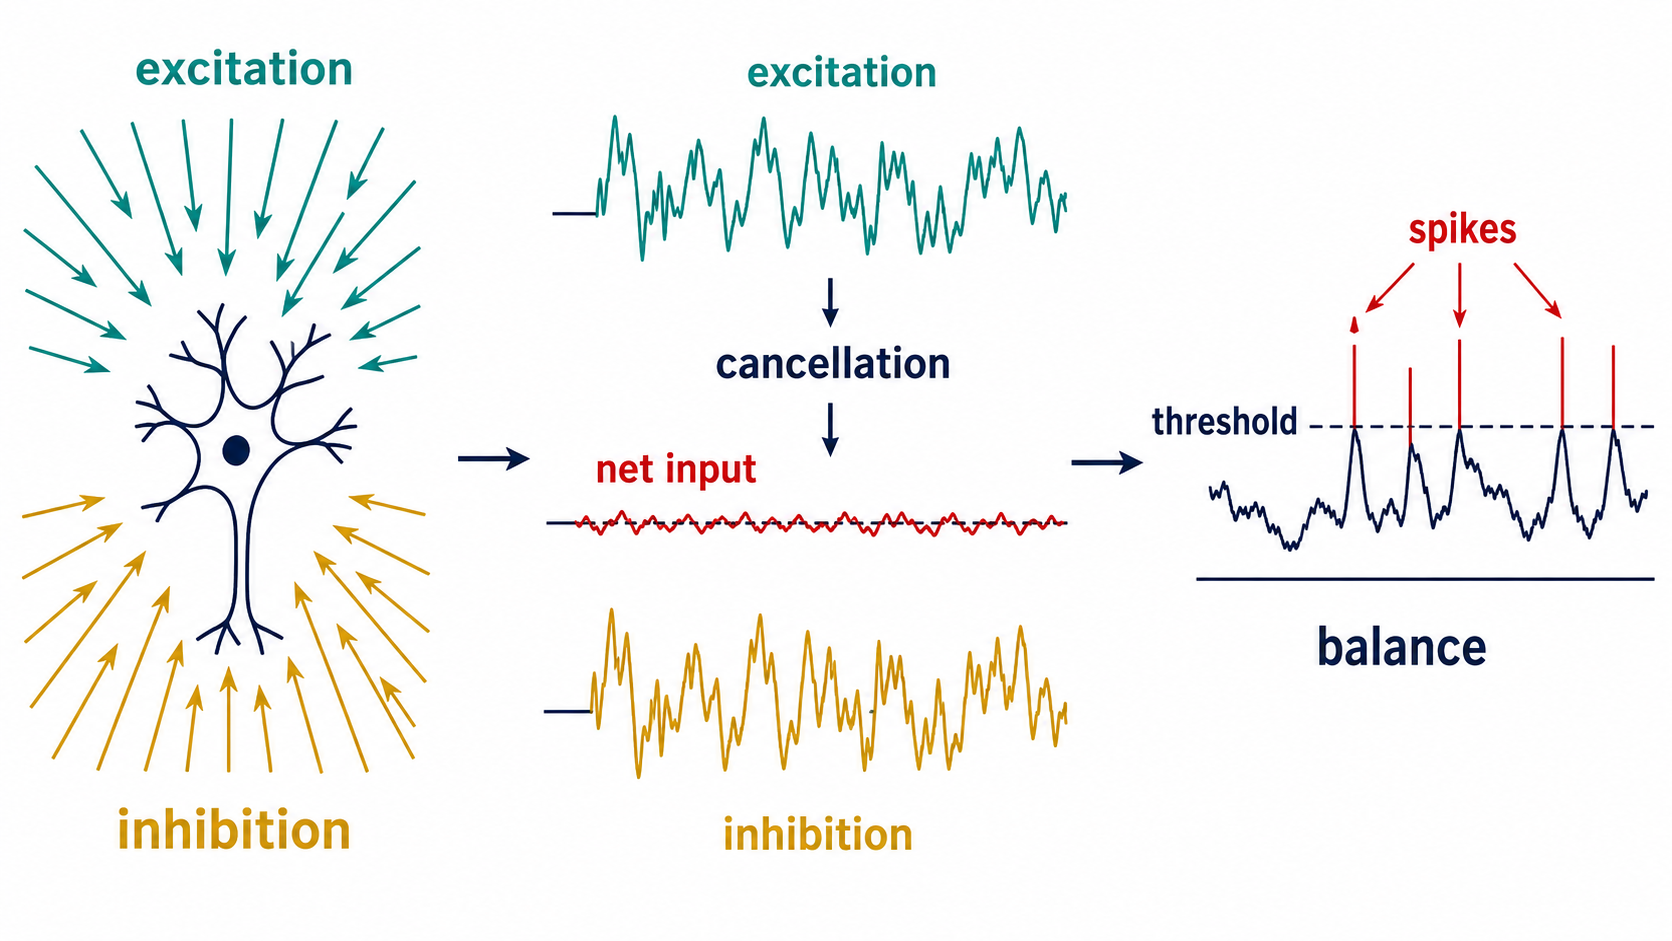
\includegraphics[width=0.92\textwidth]{figures/meso-ei-balance-cancellation.png}
\caption{Excitation-inhibition balance. Large excitatory and inhibitory currents nearly cancel in the mean, leaving a smaller fluctuating residual that drives irregular threshold crossings. The cancellation controls the operating point; the residual fluctuations control spike timing.}
\label{fig:ei-balance-cancellation}
\end{figure}

This is the central mechanism behind asynchronous irregular spiking. The network is not quiet because inputs are small. It is irregular because inputs are large, fast, and nearly cancelling.

% ============================================================
\section{Asynchronous irregular states}
\label{sec:asynchronous-irregular-states}
% ============================================================

An asynchronous irregular (AI) state has two components.

Irregular means single neurons fire with variable interspike intervals. A typical diagnostic is
%
\begin{equation}
  \operatorname{CV}_i
  =
  \frac{\sqrt{\operatorname{Var}[T_i]}}{\mathbb{E}[T_i]},
  \label{eq:ai-cv}
\end{equation}
%
where $T_i$ denotes the interspike interval of neuron $i$. Values near one indicate Poisson-like irregularity, although the process need not be exactly Poisson.

Asynchronous means the population does not fire in large coordinated volleys. If $A_a(t)$ is the population activity of class $a$,
%
\begin{equation}
  A_a(t)
  =
  \frac{1}{N_a}\sum_{i\in a}s_i(t),
  \label{eq:population-activity-ai}
\end{equation}
%
then an asynchronous state has limited population-rate oscillations and weak average pairwise synchrony.

The AI state is therefore not the same thing as independent Poisson spiking. It is a recurrent-network state in which each neuron receives fluctuating input, but the fluctuations are sufficiently decorrelated across neurons that the population rate remains comparatively smooth.

A useful local picture is
%
\begin{equation}
  \tau_m\dot V_i
  =
  -(V_i-E_L)
  +
  R_m\bigl[\mu_i+\sigma_i\xi_i(t)\bigr],
  \label{eq:diffusion-ai-neuron}
\end{equation}
%
where $\mu_i$ is the balanced residual mean and $\sigma_i\xi_i(t)$ is the fast residual fluctuation. This diffusion approximation is not the full network, but it captures why an individual cell can fire irregularly while the population remains stable.

The computation to perform is direct: plot a raster, the population rate, the ISI distribution, and the distribution of pairwise correlations. AI activity should show dense irregular rasters without coherent population bursts.

% ============================================================
\section{Mean firing rate vs spike-count variability}
\label{sec:mean-rate-vs-count-variability}
% ============================================================

Mean rate and spike-count variability are different observables. A balanced network can have stable mean rates and highly variable spike counts.

For neuron $i$, the mean firing rate over a long observation time is
%
\begin{equation}
  r_i
  =
  \lim_{T\to\infty}\frac{\mathbb{E}[N_i(0,T)]}{T}.
  \label{eq:mean-rate-definition-ch04}
\end{equation}
%
The Fano factor over a finite window is
%
\begin{equation}
  F_i(T)
  =
  \frac{\operatorname{Var}[N_i(t,t+T)]}{\mathbb{E}[N_i(t,t+T)]}.
  \label{eq:fano-definition-ch04}
\end{equation}
%
The rate asks for the average count per unit time. The Fano factor asks how reliable the count is across repeated windows or trials.

Balanced feedback primarily sets the mean operating point. Spike-count variability depends on additional structure:
%
\begin{equation}
  \operatorname{Var}[N_i(T)]
  =
  \mathbb{E}[N_i(T)]
  +
  2\int_0^T (T-\tau)\,C_i(\tau)\,\dd\tau ,
  \label{eq:count-variance-autocov}
\end{equation}
%
where $C_i(\tau)$ is the spike-train autocovariance density beyond the Poisson delta term. Positive slow autocovariance increases $F_i(T)$ at long windows. Refractoriness can decrease variability at short windows.

This distinction is essential for the clustered-network problem. Balance can explain irregular spike timing and plausible rates. It does not automatically explain super-Poisson variability over long windows. Long-window variability usually requires slow rate modulation, latent state switching, shared fluctuations, or slow cellular/synaptic variables.

% ============================================================
\section{Pairwise correlations in balanced networks}
\label{sec:pairwise-correlations-balanced}
% ============================================================

Pairwise correlations measure whether neurons fluctuate together. For spike counts $N_i$ and $N_j$ in the same window, the covariance is
%
\begin{equation}
  \operatorname{Cov}[N_i,N_j]
  =
  \mathbb{E}\!\left[
    (N_i-\mathbb{E}N_i)(N_j-\mathbb{E}N_j)
  \right].
  \label{eq:count-covariance-balanced}
\end{equation}
%
The correlation coefficient divides this covariance by the two standard deviations:
%
\begin{equation}
  \rho_{ij}
  =
  \frac{\operatorname{Cov}[N_i,N_j]}
       {\sqrt{\operatorname{Var}[N_i]\operatorname{Var}[N_j]}}.
  \label{eq:count-correlation-balanced}
\end{equation}
%
Positive $\rho_{ij}$ means the cells tend to have high counts in the same windows. Negative $\rho_{ij}$ means one tends to be high when the other is low.

Population averaging makes small correlations important. If all neurons in a population have count variance $\sigma_N^2$ and average pairwise covariance $c_N$, then
%
\begin{equation}
  \operatorname{Var}\!\left[\frac{1}{N}\sum_{i=1}^N N_i\right]
  =
  \frac{\sigma_N^2}{N}
  +
  \frac{N-1}{N}c_N .
  \label{eq:population-variance-pairwise-cov}
\end{equation}
%
The first term is private variability and vanishes as $1/N$. The second term is shared variability and does not vanish if $c_N$ remains order one.

Balanced networks can suppress average correlations through fast inhibitory feedback. A shared upward fluctuation in excitation recruits inhibition, which pushes activity back down. This negative feedback prevents the whole network from moving in lockstep.

But correlations are not guaranteed to be zero. Shared inputs, sparse connectivity, common inhibitory feedback, and structured clusters can all create correlations. For this course, the important comparison is between unstructured balanced correlations and within-cluster correlations after clustering is added.

% ============================================================
\section{Why balanced networks naturally produce irregular spiking}
\label{sec:why-balance-produces-irregular-spiking}
% ============================================================

Balanced networks produce irregular spiking because the mean input and the fluctuation scale play different roles.

The mean residual can be near threshold:
%
\begin{equation}
  \mu_i
  =
  \mathbb{E}[I_i^E+I_i^I+I_i^{\mathrm{ext}}]
  \approx
  \text{threshold-compatible drive}.
  \label{eq:threshold-compatible-drive}
\end{equation}
%
This prevents the neuron from being either silent or saturated.

The variance remains substantial:
%
\begin{equation}
  \sigma_i^2
  =
  \operatorname{Var}[I_i^E+I_i^I]
  =
  \operatorname{Var}[I_i^E]
  +
  \operatorname{Var}[I_i^I]
  +
  2\operatorname{Cov}[I_i^E,I_i^I].
  \label{eq:residual-input-variance}
\end{equation}
%
Even if excitation and inhibition cancel in the mean, their spike-timing fluctuations create a moving residual input. If the residual pushes voltage across threshold at irregular times, the output spike train is irregular.

In a fluctuation-driven regime, many spikes are caused by transient excursions rather than by a large constant suprathreshold current. That is why the same neuron can have a modest mean rate and a coefficient of variation near one.

Recurrent feedback keeps this regime self-consistent. If excitation rises too much, inhibition is recruited and pulls the residual down. If activity falls too low, inhibition also falls and excitation can recover. This feedback stabilizes rates while preserving local fluctuations.

The diagnostic prediction is specific: remove or weaken inhibition and the network should move toward runaway excitation, synchrony, or saturation. Make inhibition too strong and the network should become silent or fluctuation-poor. The balanced AI regime lives between those failures.

% ============================================================
\section{Why balanced networks alone do not give slow metastable dynamics}
\label{sec:why-balance-alone-not-metastable}
% ============================================================

Balance explains irregular spiking, but it does not by itself create a set of slow cluster states. In an unstructured random balanced network, the usual coarse picture is one stable AI operating point.

Let $\vec r(t)$ collect population rates or coarse modes around the AI state $\vec r^*$. A local linearization has the form
%
\begin{equation}
  \frac{\dd}{\dd t}\delta\vec r
  =
  \mathbf{J}_{\mathrm{AI}}\delta\vec r
  +
  \text{finite-size fluctuations},
  \qquad
  \delta\vec r=\vec r-\vec r^* .
  \label{eq:ai-linearization}
\end{equation}
%
If the eigenvalues of $\mathbf{J}_{\mathrm{AI}}$ have negative real parts bounded away from zero, perturbations decay on fast membrane, synaptic, or feedback timescales. Finite-size fluctuations then create noisy motion around one state, not long dwell times in many discrete states.

Slow metastability requires additional structure. Examples include:
%
\begin{enumerate}[leftmargin=*]
  \item clustered recurrent excitation, which creates multiple attractor-like active sets;
  \item slow adaptation or synaptic plasticity variables, which introduce slow internal state;
  \item structured low-dimensional connectivity with eigenvalues close to instability;
  \item deterministic high-dimensional chaos with slow collective modes.
\end{enumerate}
%
The Litwin-Kumar--Doiron-style baseline uses the first mechanism. Balance supplies irregular within-state spiking. Clustering supplies multiple state-dependent recurrent gains. Finite-size noise then moves the network among those states.

The central control is therefore: compare a random balanced network and a clustered balanced network with matched mean rates. If only the clustered network shows long cluster lifetimes, broad active-set occupancy, and slow cluster-rate autocorrelation, then the slow dynamics are not a generic consequence of balance.

\begin{chaptersummary}

\begin{center}
\renewcommand{\arraystretch}{1.55}
\begin{tabularx}{\textwidth}{@{}l X X@{}}
  \toprule
  \textbf{Concept} & \textbf{Equation or object} & \textbf{Interpretation} \\
  \midrule
  Balance &
  $I^E+I^I+I^{\mathrm{ext}}=\text{small residual}$ &
  Large opposing currents keep neurons near threshold \\
  Mean input &
  $\mu_a=I_a^{\mathrm{ext}}+\sum_b K_{ab}J_{ab}r_b$ &
  Population rates are constrained by cancellation \\
  Conductance balance &
  $\tau_{\mathrm{eff}}=C_m/(g_L+g_E+g_I)$ &
  Synaptic conductance changes gain and time constant \\
  Strong coupling &
  $w_{aE}=j_{aE}/\sqrt K$, $w_{aI}=-j_{aI}/\sqrt K$; $\alpha_{aE}j_{aE}r_E-\alpha_{aI}j_{aI}r_I+i_a^{\mathrm{ext}}\approx0$ &
  Leading $O(\sqrt K)$ currents cancel while $K_{ab}w_{ab}^2=O(1)$ fluctuations remain \\
  AI state &
  Irregular ISIs plus weak population synchrony &
  Single-neuron variability without population volleys \\
  Fano factor &
  $F(T)=\operatorname{Var}[N_T]/\mathbb{E}[N_T]$ &
  Count reliability is not the same as mean rate \\
  Pairwise covariance &
  $\operatorname{Var}[N^{-1}\sum_i N_i]=\sigma_N^2/N+(N-1)c_N/N$ &
  Shared fluctuations survive population averaging \\
  Missing ingredient &
  No cluster-state attractor in random balance &
  Balance gives fast irregular spiking, not slow metastability by itself \\
  \bottomrule
\end{tabularx}
\end{center}

\end{chaptersummary}

\begin{conceptquestions}
  \item Why is balance a statement about total input rather than a one-to-one matching of excitatory and inhibitory synapses?
  \item In the mean-input equation, why do excitatory and inhibitory terms cancel in the mean but not in the variance?
  \item What changes when a synapse is conductance-based rather than current-based?
  \item Explain why strong coupling can produce large excitatory and inhibitory currents but only order-one residual drive.
  \item What two empirical features must both hold for an asynchronous irregular state?
  \item Why can a neuron have a stable mean firing rate but a large spike-count Fano factor?
  \item Use \cref{eq:population-variance-pairwise-cov} to explain why tiny positive pairwise covariances can matter for population activity.
  \item How does inhibitory feedback help suppress shared fluctuations?
  \item Why does fluctuation-driven threshold crossing produce irregular spiking without requiring a slow latent state?
  \item What observation would show that slow metastability is caused by clustering rather than by balance alone?
\end{conceptquestions}

\clearpage
